\chapter{Time Discrimination-ADC -  Neyman-Pearson Detector}\label{ch:NP}
The Neyman-Pearson(NP) detector was first introduced by Jerzy Neyman and Egon Pearson in 1933\citep{neyman1933problem}, and it has been proven to be the optimal detector for radar/ laser signal detection \cite{kay1998fundamentals}. \todo{add the review to background section} 
% and has been widely utilized in many applications like target detection, medicine, nuclear energy, gravitational-wave astronomy, \etc\cite{Hoover2000LocatingResponse,Bousselham2007SamplingTiming,seto2001possibility,gronwall2007influence,gu2002detecting,Jordan2009RangeData,roman2000parametric,Ofek2017OptimalDetection,Vio2018MatchedImplementation}. 
In general, the NP detector conducts a likelihood ratio test(LRT) to detect a known deterministic signal, \ie the signal has no unknown parameters, while in our case, the arrival time and the amplitude of the return pulse are unknown. In that case, a generalized likelihood ratio test(GLRT) is utilized for detection of signals that have unknown parameters. Moreover, the arrival time of signals can also be determined in the detection process, so our signal detection and estimation problem are combined together, and the problem is defined in the next.
%% problem definition
\section{Problem definition}
We state the signal $x[n]$ collected by an ADC is composed of a Gaussian distributed white noise under hypothesis $\hzero$, and under hypothesis $\hone$ the signal is the summation of the noise-free return pulse with unknown amplitude, $As[n]$, and white noise following a  Gaussian distribution. Symbolically,
\begin{align}\label{eq:mf_hypothesis}
\mathcal{H}_0:x[n]&=w_0[n]  &n=0, 1,\ldots, N-1\\
\mathcal{H}_1:x[n]&=As[n-n_0]+w_1[n]  &n=0, 1,\ldots, N-1    
\end{align}
where $w_0$ and $w_1$ are the white noise under $\hzero$ and $\hone$ with the variance $W$, and $s$ is the template of the transmit signal normalized to unit amplitude which is also called 'kernel'. The kernel is scaled by the unknown amplitude $A$ and it is assumed to be nonzero over the time interval $[0,M-1]$. The index $n$ represents the timestamp of the $n$-th point of the signal with a size of $N$, and $n_0$ stands for the arrival time of the signal. The time period $[0, N-1]$ should cover the signal for all the possible arrival time, \ie $n_0\in[0, N-M]$. \par
Note in Equation \eqref{eq:mf_hypothesis}\todo{change eq No.}, the noise on each point of a signal is approximated to be Gaussian distributed, even though the shot noise is created with a Poisson distribution. This approximation is explained in \citep{wall1979practical} who states that, despite the number of photons follows Poisson statistics, after sufficient integration for a photon detector of more than 10 photons per integration time interval, the distribution is reduced to Gaussian. In our case, the collected number of photons is far beyond 10 when the laser is on, so the Gaussian approximation is valid. In addition, the white noise $w_0$ and $w_1$ usually have different variances because the shot noise induced by the laser pulse also contributes to the variance of $w_1$. However, the $W_1$ is usually unavailable since the pulse-induced shot noise is amplitude depended which is unknown, and the unknown amplitude also makes it difficult to measure the variance of the pulse-induced shot noise with the appearance of the pulse. Therefore, in this study the $w_0$ and $w_1$ are assumed to be identical, denoted by $w$, and they share the same variance $W$. Also. we can see this approximation does not affect the PFA, and has negligible influence on the PD in next few sections. \par
Next, we introduce the Neyman-Pearson theorem which allows us to decide the hypothesis of a signal.
% NP theorem
\subsection{Neyman-Pearson Theorem}
The Neyman-Pearson theorem (NP theorem) states that, to maximize the probability of detection (PD) $P_D$ of a signal for a given probability of false alarm (PFA) $P_{fa}  =\alpha$, decide $\mathcal{H}_1$ if the generalized likelihood ratio $L_G(x)$ is greater than a threshold $\gamma$; otherwise, decide $\mathcal{H}_0$:
\begin{equation} \label{eq:Lx}
L_G(x)=\frac{p(\vec{x};n_0,A,\mathcal{H}_1)}{p(\vec{x};\mathcal{H}_0)}\underset{\mathcal{H}_0}{\overset{\mathcal{H}_1}{\gtrless}}\gamma
\end{equation}
The threshold $\gamma$ can be derived from the definition of the PFA
\begin{equation}\label{eq:pfa}
P_{fa}=\int_{\{\vec{x}:L_G(x)>\gamma\}} p(x;\mathcal{H}_0)dx=\alpha,
\end{equation}
and the PD can be obtained by:
\begin{equation} \label{eq:pd}
P_D=\int_{\{\vec{x}:L_G(x)>\gamma\}}p(x;n_0, A, \mathcal{H}_1)d\vec{x}
\end{equation}
The probability density distribution (PDF)  of signals with unknown parameters $n_0$ and $A$ under hypothesis $\hzero$ and $\hone$ are denoted by $p(\vec{x};n_0, A,\mathcal{H}_1)$ and $p(\vec{x};\mathcal{H}_0)$, respectively, and the vector $\vec{x} = [x[0],x[1],...,x[N-1]]$. The generalized likelihood ratio indicates the likelihood of a signal being $\hone$ versus being $\hzero$, and Inequation \eqref{eq:Lx} is called the generalized likelihood ratio test. After mathematical reorganization, the GLRT is reduced to (the derivation is provided at the end of this chapter.\todo{ref the last page of this chapter}):
\begin{eqnarray} \label{eq:Tx}
T(x) &=&\sum_{n=n_0}^{n_0+M-1}x[n]s[n-n_0] \underset{\mathcal{H}_0}{\overset{\mathcal{H}_1}{\gtrless}}\gamma'\\
\gamma'&=&\frac{A}{2}\sum_{n=0}^{M-1}s^2[n]+\frac{W\ln\gamma}{A}
\end{eqnarray}
and Equation\eqref{eq:pfa} is reformed to
\begin{equation}\label{eq:pfa2}
P_{fa}=Pr(T(x)>\gamma';\mathcal{H}_0)
\end{equation}
where $T(x)$ is the test statistic which needs to be calculated from experiments. Equation\eqref{eq:Tx} indicates the GLRT calculates the cross-correlation of the signal $x$ with the kernel $s$ for all possible $n_0$, and compares the maximum value with the threshold $\gamma'$. If the threshold is exceeded, a pulse is claimed to be present, and the arrival time $n_0$ is equal to the timestamp of the maximum value. Otherwise, noise is claimed detected. Mathematically, the test statistic can also be written as
\begin{align}\label{eq:MF_Tx_argmax}
    T(x)&=\max_{n_0\in[0,N-M]}\sum_{n=n_0}^{n_0+M-1}x[n]s[n-n_0]\\
    n_0&= \argmax_{n_0\in[0, N-M]}T(x)
\end{align}
In practice,  $T(x)$ can be obtained from the convolution of a signal with the conjugated time-reversed kernel $s'[n]$, \ie for each timestamp $n$, the convolution result is
\begin{align}\label{eq:MF_conv}
y[n]&=\sum_{m=0}^nx[m]s'[n-m]\\
s'[n]&=s[N-1-n]
\end{align}
and Equation\eqref{eq:MF_conv} is also known as the \emph{matched filter} (MF). For simplicity, this detection algorithm is called NP detector in this work. The NP detector is proved mathematically equivalent to the correlation between the signal and the kernel. For the difference between the correlation approach and the NP detector readers could refer to [Kay, book]\todo{add kay book Vol II}for details.
\subsection{Fast Fourier Transformation Approach}
The NP detector can be achieved by sliding the kernel over an input signal in time domain. The time complexity of the temporal convolution approach can be denoted by $\mathcal{O}(MN)$ in which $M$ and $N$ are the number of points of the kernel and the signal, respectively. Therefore, the MF could be computationally intensive if the signal contains a large number of data points. Alternative solution is needed to accelerate the computation. As we know that the convolution of two signals in time domain is equivalent to a dot product of the Fourier Transformation of the two signals in frequency domain, the Equation~\eqref{eq:MF_conv} can be implemented in frequency domain by using Fast Fourier Transformation (FFT). Specifically, 
\begin{align}
X&=\mathcal{F}[x]\\
S&=\mathcal{F}[s]\\
Y&=X\cdot S\\
y&=\mathcal{F}^{-1}[Y]
\end{align}
where the variable $X$, $S$, and $Y$ are the Fourier Transformation (FT) of the signal $x$, $s$ and $y$ in frequency domain, and the symbol $\mathcal{F}$ and $\mathcal{F}^{-1}$ are the FT and inverse-FT operators. The time complexity of an FFT operation is $\mathcal{O}(N\log N)$ which is much smaller than $\mathcal{O}(MN)$. Another benefit of using FFT is that arrival time smaller than the ADC sampling interval can be resolved by using zero-padding technique. In other words, the temporal resolution of the convolution results can be improved.\ par
The zero-padding technique is to add zeros to signals in time or frequency domain), and the sampling rate of signals in frequency or time domain increases after FT or inverse-FT. For an FFT operation without zero-padding, since the number of points in frequency domain is equal to the number of data points used in the FFT in time domain, the resolution of the signal is unchanged, \ie no improvement is on the resolution. On the contrary, for a signal having $N$ points (sampling rate of $1/N$) in time domain, if $N$ zeros are padded at the end of the signal in frequency domain (assuming the frequency is centered around zero), the signal will have $2N$ points after inverse-FT. And since the time range is unchanged, the resolution of the signal is doubled. On the other hand, the FFT is most efficient when the number of points of a signal is an integer power of two, which means zero padding in time domain is also needed for signals have variable sizes, and note that the time-domain zero-padding only extends the length of the signal but does not increase the signal resolution. In this work, we first zero-pad the signal $s$ and $x$ to an identical length $L_{p2}$ which is the smallest power of two of the total length ($M+N-1$) of the two signals. After FFT, we add $K$ zeros to the dot-product result $Y$, and $K$ is an integer times the length $L_{p2}$. After the zero-padding in frequency domain, the size of the resultant signal is extended to $(K+1)L_{p2}$, and then the resultant signal is converted back to time domain and the size of the signal is unchanged. The convolution result $y$ has additional zeros which results from the time-domain zero-padding at the first step, so the zeros are removed from the convolution result. After the zero-removal, the size of the convolution result becomes $(K+1)(M +N-1)$, \ie the resolution increases $K+1$ times than the sliding-window convolution. Accordingly, the original time interval $\Delta t$ is reduced to $\Delta t/(K+1)$. Note that the size of the convolution result is larger than the time series, so only the center portion of the convolution result is kept to maintain the size consistency. An example of the zero-padding in time domain and in frequency dodfdffmain is shown in Figure ~\ref{fig:ADC_NP_zeropad}. The time is arbitrary. In Figure~\ref{fig:ADC_NP_zeropad} (c), we can see the resolution of the convolution result is double after frequency-domain zero padding.
\begin{figure}[t!p]
\centering
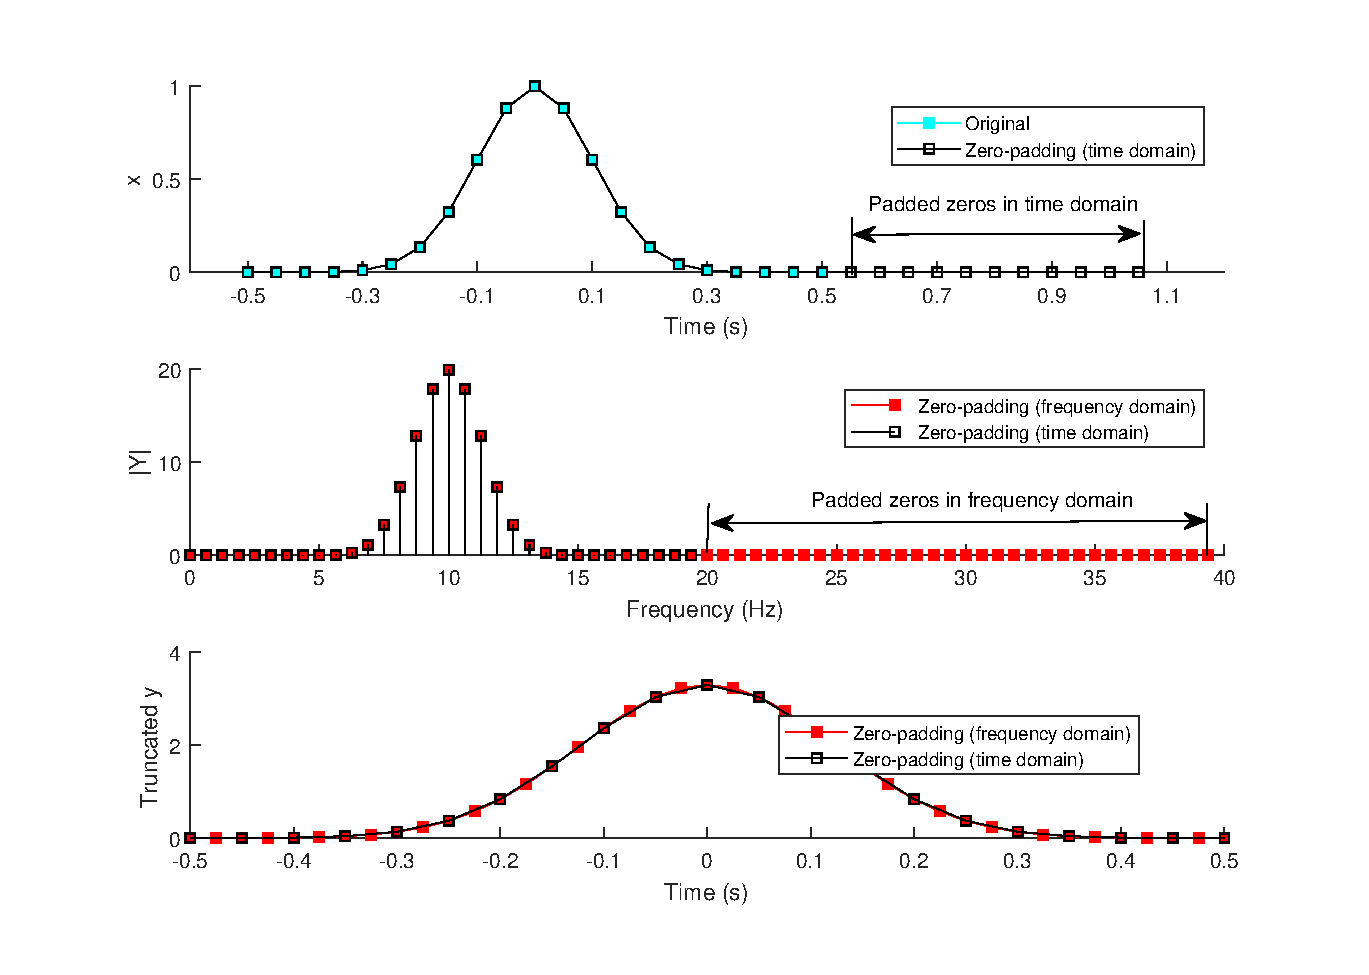
\includegraphics[width=0.8\textwidth]{figures/chapter_ADC_MF/signal_pad_nopad.eps}
\caption{Example of zero-padding in time domain and frequency domain}
\label{fig:ADC_NP_zeropad}
\end{figure}
% PDF
\subsection{PDF of $T(x)$}
Now, the original GLRT (Equation \eqref{eq:Lx}) is reduced to a problem that compares the $T(x)$ with a new threshold $\gamma'$ (Equation\eqref{eq:Tx} and Equation \eqref{eq:MF_Tx_argmax}). Now, we need to determine the threshold $\gamma'$ using Equation \eqref{eq:pfa2} for a given $P_{fa} = \alpha$, for which the PDFs of $T(x)$ under both hypothesis $\hzero$ and $\hone$ are required. Since $T(x)$ is a linear combination of Gaussian distributed variables, the PDFs of $T(x)$ should also follow a Gaussian distribution. The estimation of the mean $\hat{\mu}$ and the variance $\hat{\sigma}^2$ for hypothesis $\hzero$ and $\hone$ are shown below, of which the derivation is given at the end of this chapter\todo{refer to last page of the chapter}:
\begin{align} \label{eq:pdfTx}
\hat{\mu_0}&=0\\
\hat{\sigma_0^2}&=W\sum_ns[n]^2\\
\hat{\mu_1}&=A\sum_ns^2[n]\\
\hat{\sigma_1^2}&=W\sum_ns^2[n],
\end{align}
and the PDFs of $T(x)$ follow:
\begin{align}
\mathcal{H}_0: & T(x)\sim N(\hat{\mu_0}, \hat{\sigma}_0^2)\\
\mathcal{H}_1: & T(x)\sim N(\hat{\mu_1}, \hat{\sigma}_1^2)
\end{align}
Or, the normalized test statistic $T'(x) = \frac{T(x)-\hat{\mu}}{\hat{\sigma}^2}$ follows the standard normal distribution $\mathcal{N}(0,1)$.
% threshold
\subsection{Estimation of threshold $\gamma'$}
Having the PDF of $T(x)$, Equation \eqref{eq:pfa2} can be expressed by
\begin{align} \label{eq:pfa_gamma}
\begin{split}
P_{fa}&=Pr(T(x)>\gamma';\mathcal{H}_0)\\
&=Pr(T'(x)>\frac{\gamma'-\hat{\mu}_0}{\hat{\sigma}_0};\mathcal{H}_0)\\
& = Q(\frac{\gamma'-\hat{\mu}_0}{\hat{\sigma}_0})
\end{split}
\end{align}
where 
\begin{align}
\begin{split}
Q(x) &=\int_x^\infty\frac{1}{\sqrt{2\pi}}\exp(-\frac{1}{2}t^2)dt\\
&=\frac{1}{2}[1-erf(\frac{x}{\sqrt{2}})]\\
&=\frac{1}{2}erfc(\frac{x}{\sqrt{2}})\\
&=1-\Phi(x)
\end{split}
\end{align}
and $\Phi(x)$ is the cumulative distribution function(CDF) for a standard normal distributed variable, and $Q(x)$ is the complementary cumulative distribution function(CCDF). Then, we can derive the expression of $\gamma'$
\begin{align} \label{eq:MF_gamma'}
\gamma'=\hat{\sigma}_0Q^{-1}(P_{fa})+\hat{\mu}_0    
\end{align}
Here, we can see the PFA is not a function of the amplitude $A$ or the variance of $\hone$signal $w_1$, which means the amplitude of a signal and the variance will not affect the FPA. However, the PD could be affected. The theoretical PD can be obtained from \eqref{eq:pd}
\begin{align}
\begin{split} \label{eq:MF_pd}
P_d&=Pr(T(x)>\gamma';n_0,A, \mathcal{H}_1)\\
&  = Pr(T'(x)>\frac{\gamma'-\hat{\mu}_1}{\hat{\sigma}_1};n_0,A, \mathcal{H}_1)\\
& = Q(\frac{\gamma'-\hat{\mu}_1}{\hat{\sigma}_1})\\
&=\frac{1}{2}erfc(\frac{\gamma-\hat{\mu}_1}{\sqrt{2}\hat{\sigma_1}})
\end{split}
\end{align}
Plugging Equation \eqref{eq:MF_gamma'} in Equation \eqref{eq:MF_pd}, we have
\begin{align} \label{eq:MF_deflectCoef}
P_d &= Q(Q^{-1}(P_{fa})-\sqrt{d^2})\\    
d^2 &= \frac{A^2s^2[n]}{W}
\end{align}
where $d^2$ is the deflection coefficient, which can be interpreted as the normalized difference between the PDF of $T(x)$ under hypothesis $\hone$ and hypothesis $\hzero$ by the variance of the noise. The deflection coefficient illustrates that the separation between the two PDFs, as shown in the schematic Figure \ref{fig:dsquare}. In the case of the deflection coefficient is large, the position of the threshold has less impact on the PD, and the detector is approaching a perfect detector($PD = 1$). However, as shown in Equation \eqref{eq:MF_deflectCoef} the deflection coefficient is a function of the amplitude $A$ and variance $W$of a signal, which means the smaller amplitude and larger variance could move the two PDFs closer which causes a decrease of PD.
\begin{figure}[t!p]
\centering
\includegraphics[width=.8\textwidth]{figures/chapter6_ADC/dsquare.jpg}
\caption{PDF of $\hzero$ and $\hone$, and the deflection coefficient [Ref [Kay book]]}
\label{fig:dsquare}
\end{figure}
% Procedure
\subsection{Procedure of the NP detector}
Now, we have the problem defined and also the PDFs and the threshold derived. To summarize, the procedure of the NP detector for the signal detection and estimation is following:
\begin{enumerate}
\item Find the kernel $s[n]$;
\item Find the STD of noise $x[n]$;
\item Calculate the PDFs of the test statistic T(x): Equation \eqref{eq:pdfTx}; \todo{change equation label}
\item Calculate the threshold $\gamma'$ (threshold for $T(x)$): Equation\eqref{eq:MF_gamma'};
\item Calculate the $T(x)$ over all possible $n_0$ by convoluting the input signal $x$ and the kernel $s$, and find the maximum value of $T(x)$ and the corresponding $n_0$: Equation\eqref{eq:MF_Tx_argmax} and Equation \eqref{eq:MF_conv};
\item Compare the maximum value of $T(x)$ with the threshold $\gamma'$, and decide the hypothesis of the signal: Equation \eqref{eq:Tx};
\item If $\hone$, estimate the arrival time $n_0$: Equation \eqref{eq:MF_Tx_argmax}.
\end{enumerate}
%% Application to simulated signals 
\section{Application to simulated signals}
In this section, the application of the MF to noise signals and pulse signals was studied. The experiment design will be introduced first followed by the results and discussion.\par
\subsection{Study cases}
A case with pure noise signals and one with noisy return pulses were studied in this work. For both cases, the ADC threshold was set 3x noise floor above zero, and the edge-trigger model with a precursor length of 1 and collection length of 5 was used. More details of the two cases are explained below.
\subsubsection{Case 1: Noise (laser is off)}
For the case of noise, 1000 observation of pure noise signals (with lase turned off) were generated by the noise model with a sampling rate of 100GHz as suggested in the Pulse Model section. In the noise model, the background and dark-current induced shot noises were at first generated at each data point following a Poisson distribution and then smoothed by a moving average with a kernel size of 5. The moving average is to model the APD integration process, and the size of 5 is determined by the integration time of the APD. The APD used in this study has a bandwidth of 10GHz, so the integration frequency is 2x10GHz (the integration time is 1/20GHz or 0.05ns), which results in the size of 5 for the averaging window. Next, the noise signals were subsampled with a rate of 2.5GHz to model the sampling process of an ADC with a sampling rate of 2.5GHz for the two-channel mode. 
\subsubsection{Case 2: Pulse}
Return signals reflected from targets at different distances were tested for the case with the laser on. The distance ranges from 5m to 60m with an increment of 5m and the corresponding SNR ranges from 44.4dB to 1.27dB. For each distance, 1000 return signals were generated by the pulse model, the propagation model, and the noise model. The process of moving averaging and subsampling is the same as in Case 1. 
% Detection and Estimation Algorithm: NP detector (MF) 
\subsection{Detection and Estimation Algorithm: NP detector (MF)}
The NP detector was used for the signal detection and TOF calculation. The kernel of the NP detector was obtained from the pulse model with the amplitude normalized to one. The PFA is set to 0.001 which is a typical value for a laser range finder \citep{burns1991system}. In Case 1, the variance $W$ is calculated dynamically from each observation, meaning the threshold is dynamic for the MF. In Case 2, as mentioned in Section (principle section), the variance $\sigma^2_1$ is assumed to be equal to $\sigma^2_0$, \ie $\sigma^2_1= \sigma^2_0 = W$. The PDFs of the $T(x)$ and the threshold can be obtained from Equation \eqref{eq:pdfTx}.
% % Discussion
\subsection{Results and Discussion}
\subsubsection{Threshold}
The threshold for the MF is determined by the STD of the $\hzero$ signals, $\sigma^2_0$, and different ways of calculating the STD results in different PFAs. The STD of noise signal can be obtained from the datasheet of an electronic device or measurement of an oscilloscope or signals collected by an ADC. A comparison of the STD obtained from signals before ADC sampling (analogy to oscilloscope measurements) and after sampling (analogy to signals collected by an ADC) is shown in Figure 1. The figure shows the before-sampling signals have a smaller STD compared to after-sampling signals, which results in a lower threshold, and consequently a high PFA. The reason for the difference of the STD is that the ADC only samples a limited number of data points from analog signals, and the variance of the subset of a signal is usually higher than the one of the analog signals. Consequently, the threshold for a given PFA is underestimated by using the STD of before-sampling signals. Therefore, to achieve the given PFA, the STD of the $\hzero$ signals should be calculated from the signals collected by an ADC, rather than before the ADC sampling, from oscilloscope measurements or the datasheet of an electronic device. 
% Figure 1 The STD of 1000 noise signals before ADC sampling (red) and after ADC sampling (blue).
\subsubsection{Probability of false alarm}
Monte-Carlo experiment was performed on 100 tests, each of which contains 1000 observations. The PFA of each test was measured the average PFA was obtained by averaging over the PFAs of the 100 tests. The resultant $P_{FA,aveg} $is equal to 0.08 with an STD of 0.025. The measured PFA is higher than the predefined value (0.001) because the defined threshold is for an LRT on signals with known arrival time, but the arrival time is unknown in our study. Therefore, a convolution over the entire signal is required, in which case the random noise on the signal has a much higher probability to exceed the threshold and be detected as a pulse.
\subsubsection{Probability of detection}
All the signals in Case 2 give a $P_D=1$. This is because even though the PD is theoretically dependent on the amplitude of the signal Equation \eqref{eq:MF_deflectCoef}, the deflection coefficient is large, even for signals with a low SNR. A signal observation with an SNR of 1.31dB is shown in Figure 2 along with the convolution results and the threshold. In the example, the square root of the deflection coefficient ($d = 15.7$) is much larger than the normalized threshold ($\gamma '/\sigma_0 = 3.09$), which means the PDF of hypothesis $\hone$ is separated from the one of hypothesis $\hzero$. One can also use the MLE to estimate the amplitude of the signal to reduce the effect of the amplitude on the PD \citep{kay1998fundamentals}: 
\begin{equation}
    A =\frac{\sum_{n=0}^{N-1}x[n]s[n]}{\sum_{n=0}^{N-1}s^2[n]}
\end{equation}
However, since the PD is already equal to 1 in our case, the MLE estimation is skipped, but it could be an option for readers who have situations that have a smaller amplitude, and a high PD is requested.
% Figure 2 Simulated signal with an SNR of 1.31dB with its convolution result and threshold. The maximum value of the convolution result is still higher than the threshold
\subsubsection{Accuracy and Precision}
The mean error and the RMS error are calculated to evaluate the performance of the MF. Both the sliding-window and the FFT approaches were applied. Also, to reduce the effect on the noise on the measurement, a Butterworth low-pass filter with cutoff frequency of 0.4GHz and sampling rate of 2.5 GHz was applied \todo{more details of the LP filter will be given in Section xx},The results are shown in Figure~\ref{fig:error_NP_sim}. 
 \begin{figure}[t!p]
\centering
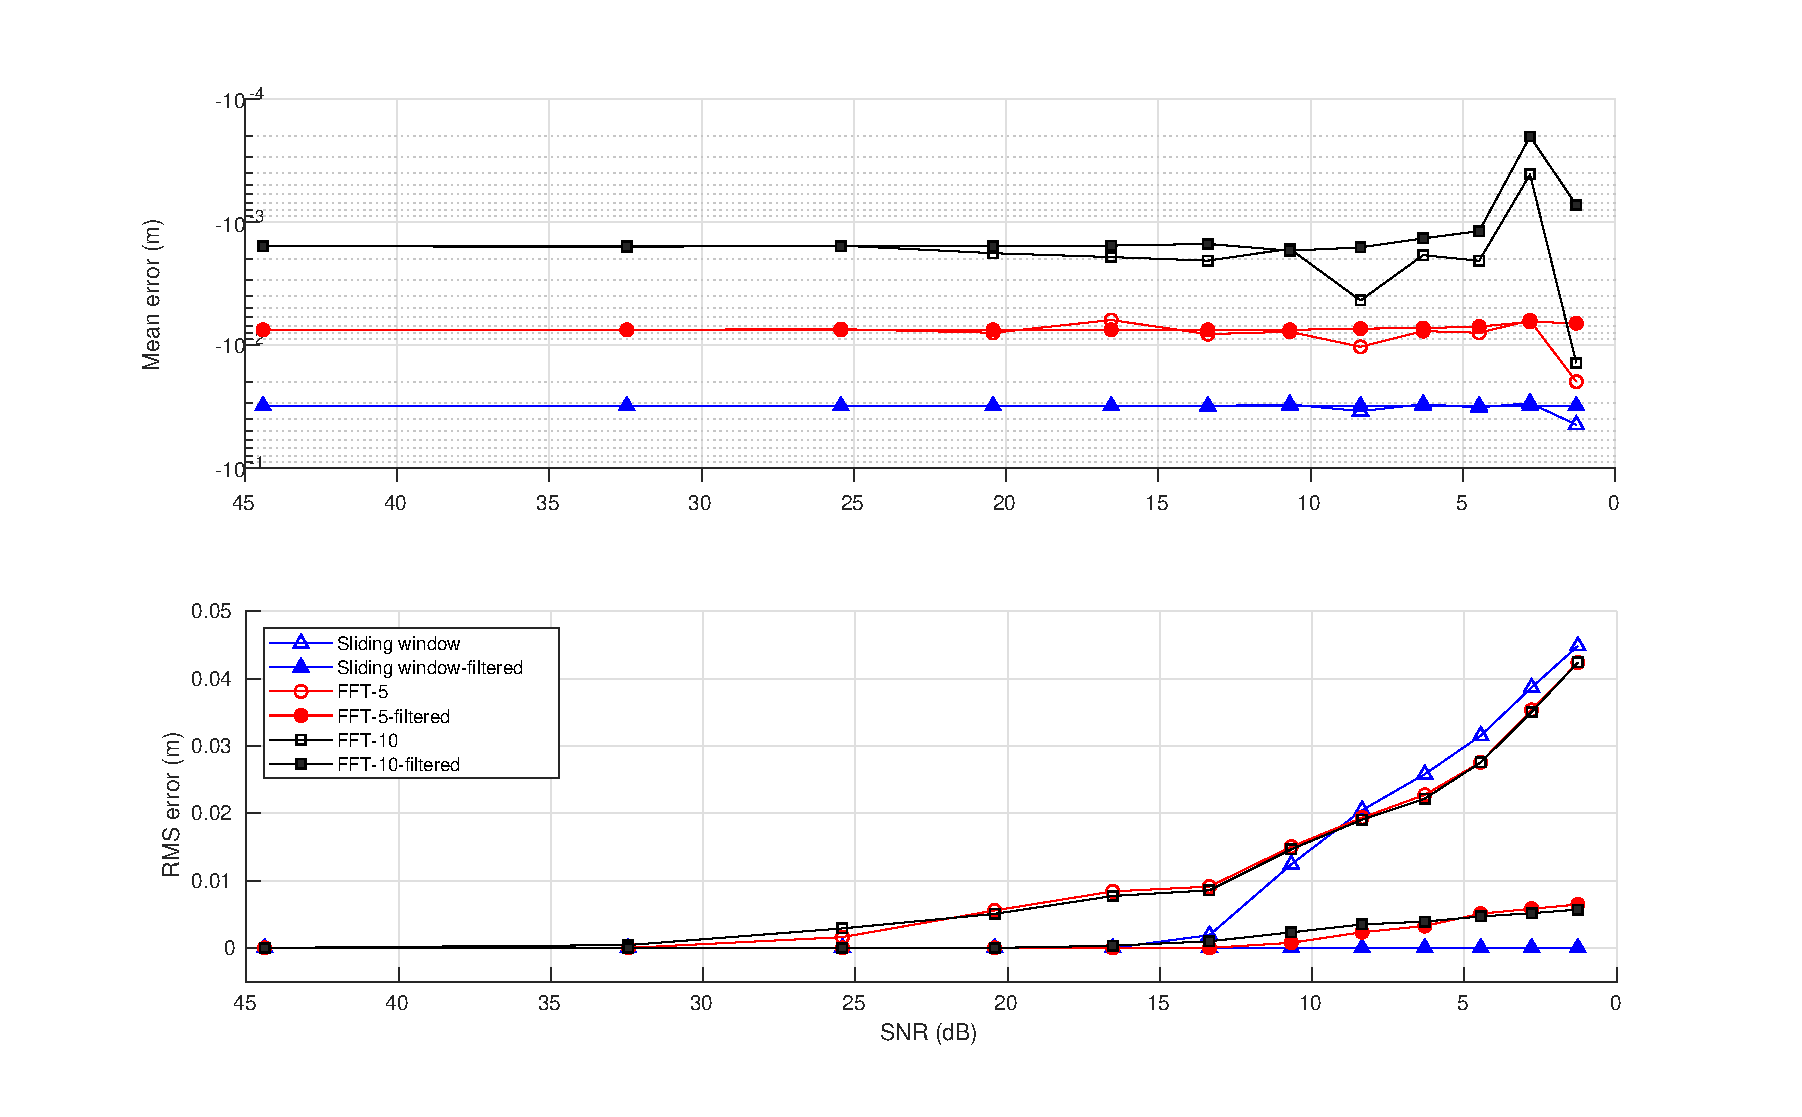
\includegraphics[width=1\textwidth]{figures/chapter_ADC_MF/Error_convVsFFT_filt_unfilt_sim.eps}
\caption{Mean and RMS error of the NP detector using the SW and FFT approaches. The number after FFT indicates the times the resolution is refined. The hollow marker indicates the results without filtering, and the solid marker denotes the result after filtering}
\label{fig:error_NP_sim}
\end{figure}
From the result of the Mean error, we can see the sliding window approach has a larger error than the FFT approach, and larger number of zero-padding gives better accuracy. The reason is that the Mean error is affected by the resolution of the signal. The sliding-window approach has the coarsest resolution, so any errors caused by the noise is at least 0.4 ns (0.06m). On the contrary, the FFT-approach refines the resolution 5 and 10 times than the sliding-window approach, which results in a less Mean error and the FFT-10 provides the least Mean error. Additionally, the LP-filtering slightly reduces the Mean error for long distance. The comparison of the effect of the resolution on the measurement accuracy between different approaches is given in Figure~\ref{fig:NP_sig_FFT5} and Figure~\ref{fig:NP_sig_FFT10}. From the figure we can see because of the finer resolution, the peak position of FFT-10 is closer to the ground-truth position than FFT-5, and the peak position of the sliding-window approach has the largest separation from the ground-truth. \par
\begin{figure}[t!p]
\centering
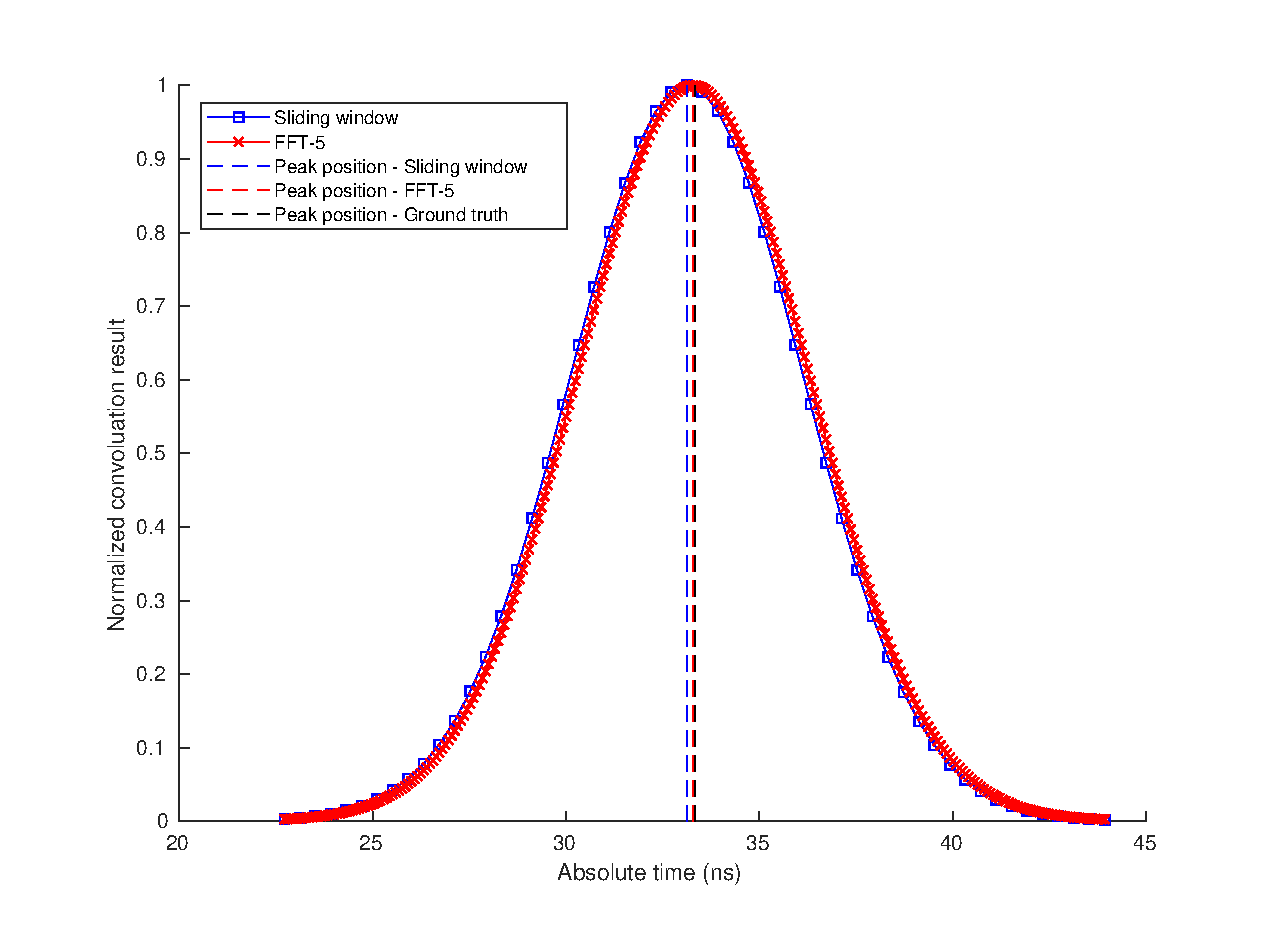
\includegraphics[width=1\textwidth]{figures/chapter_ADC_MF/plot_convRes_FFT5_sim.eps}
\caption{Convolution result of FFT-5}
\label{fig:NP_sig_FFT5}
\end{figure}
%
\begin{figure}[t!p]
\centering
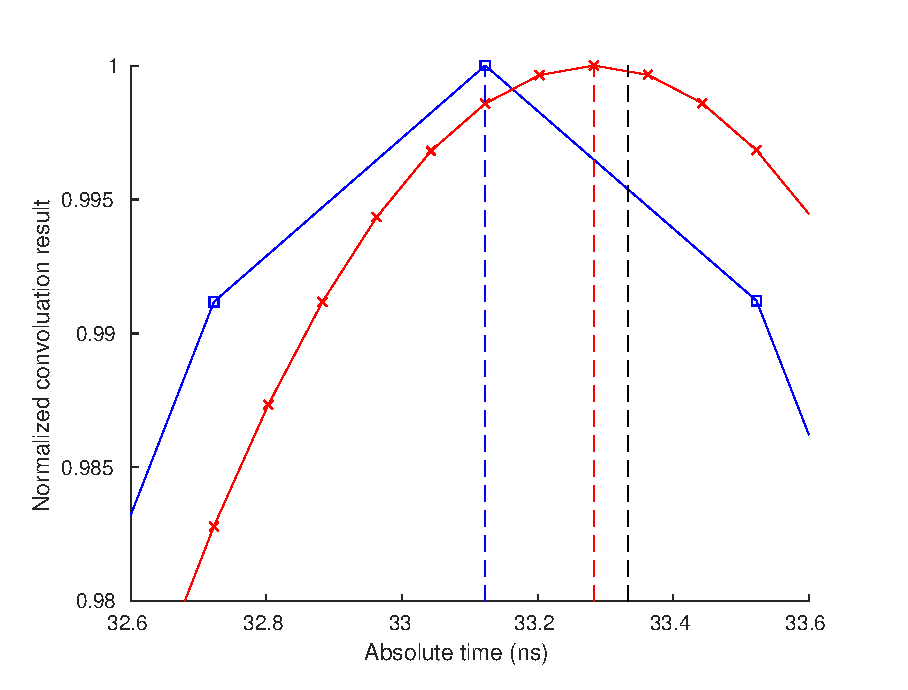
\includegraphics[width=1\textwidth]{figures/chapter_ADC_MF/plot_convRes_FFT5_zoomin.eps}
\caption{Convolution result of FFT-5 zoom in}
% \label{fig:NP_sig_FFT5}
\end{figure}
%
\begin{figure}[t!p]
\centering
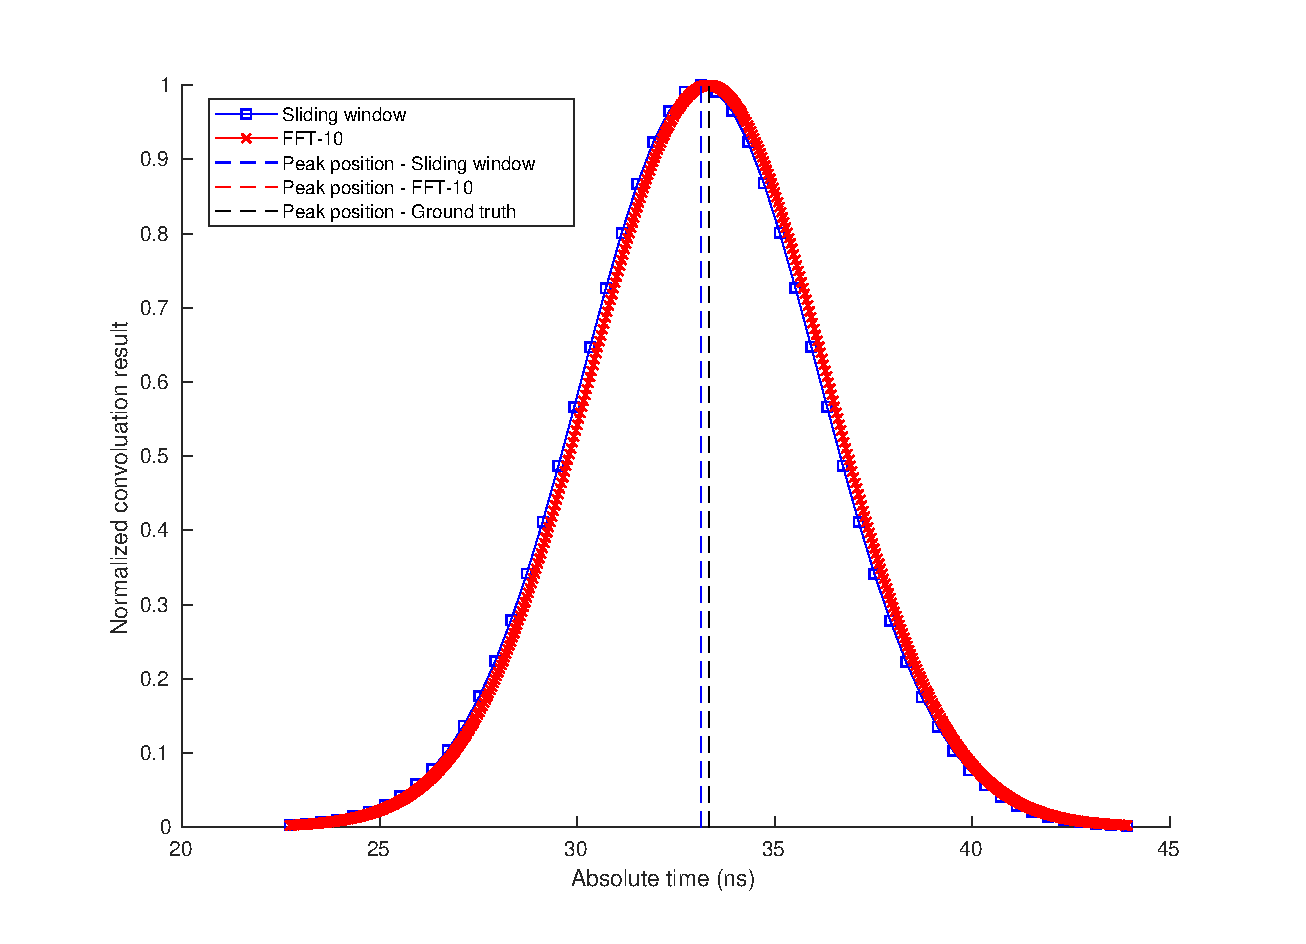
\includegraphics[width=1\textwidth]{figures/chapter_ADC_MF/plot_convRes_FFT10_sim.eps}
\caption{Convolution result of FFT-10}
\label{fig:NP_sig_FFT10}
\end{figure}
%
\begin{figure}[t!p]
\centering
\includegraphics[width=1\textwidth]{figures/chapter_ADC_MF/plot_convRes_FFT10_zoomin.eps}
\caption{Convolution result of FFT-10 zoom in}
% \label{fig:NP_sig_FFT10}
\end{figure}
From the RMS error, we notice that the sliding-window has a better precision than the FFT-approaches for shorter distance, but the precision becomes worse as the distance increases. The difference is also caused by the resolution of the result. At short distance, the signal is less noisier and the samples of a signal are more separated for the sliding-window approach than the FFT's, so the peak of the convolution result is less challenged by the adjacent points, which results in smaller variation of the time(distance) calculation. On the contrary, the samples at the top portion of the signal are likely have similar values for the FFT approaches, due to the smaller separation between the sample points, which results in a larger variation of the peak position, and consequently, larger RMS error. On the other hand, as the distance increases, the signal becomes noisy, so the values at the top portion of the result from the SW-approach also become competitive, which results in an increase of the variation of the peak position. Therefore, the larger time interval between the samples of the SW approach than the FFT approaches results in a larger RMS error of the former one. Moreover, the LP-filter improve the precision of both approaches (the RMS errors reduce to less than 1cm). Also, note that the RMS error of the SW approach becomes smaller than the one of the FFT approaches at longer distance. It is because the LP filter reduces the noise of the signal, which makes the adjacent points at the top portion of the result of the SW approach less competitive (similar to the situation for short distance). Therefore, the variation of the peak position of the SW approach decrease.
% Application to simulated data
% Mean error (1)slidng > FFT-5 > FFT-10, due to finer resolution

% RMS error (1) shorter distance sliding window < FFT. Reason is  the peak is not very noisy at shorter distance, and sliding window has coarse resolution,so  ajacent points to the peak is less likely to have competetive value to the peak. so RMS is less. For FFT, the resolution is high, so the ajacent poits could have value equal or higher than the peak, so some variaion. 

% at larger distance, the signal becomes noisy,  the adjacent points has larger fluctuation which starr to affect the sliding window, and because of the larger time interval, the RMS is larger than the variation of FFT

% (3) the LP filter remove the noise on the signal --> signal becomese smooth, so the  situation becomes similar to the short distance case: the ajacent points has less change to chanllage the peak position, so the RMS is less. Howerver, the high resol of FFT --> higher RMS. BUT, all the RMS is less than 1cm !!!
 %%%
%%
% Application to real signals
\section{Application to real signals}
The MF was also applied to real signals collected by the ADC installed on the prototype lidar. The experiment design including the experimental setup will be introduced first in this section, followed by the results and discussion.
\subsection{Experimental setup}
The setups for ADC and oscilloscope experiment are given below. The RF attenuator for the ADC experiment is to reduce the return voltage less than the upper limit of the ADC input.
\textbf{Oscilloscope}
\todo{add setup figure}
% NPL → EYDFA → 1% tap → PR-10 → oscilloscope (START channel) 

%           → 99% → Collimator → free-space → APR → oscilloscope (STOP channel) 

% ADC 

% NPL → EYDFA → 1% tap → PR-10 → ADC (START channel) 

%           → 99% → Collimator → free-space → APR →RF 20dB attenuator → ADC (STOP channel) 

\subsection{Study cases}
\subsubsection{Case 1: Noise (laser is off)}
For Case 1, the ADC threshold was set 3x noise floor above zero, and the edge-triggering with precursor length of 5 and collection length of 40 were used. The settings guarantee sufficient data points are collected in each observation. During the experiment, there are 67370 noise signals with laser off that were collected from the START channel of the ADC and 73133 noise signals collected from the STOP channel. The signals from the START and STOP channels suffer from different types of noise in addition to the regular white noise as mentioned before. The START channel signals are subject to a randomly occurring time-structured noise, which is named Hump-Noise hereinafter because of the shape. Figure 4 illustrates examples of the different types of noise on the START signal.
% Figure 4 Different types of noise on the START signal: (a) regular white noise, (b) Hump-Noise + regular white noise.
The STOP signals suffer from two frequency-structured noises with a frequency of 3.75MHz and 645MHz, which are named 3.75MHz-Noise and 645MHz-Noise, respectively. In addition, the STOP signals are subject to a Hump Noise. In the STOP channel, the 645MHz noise has a constant appearance on the signals, while the 3.75MHz-Noise and the Hump Noise occurs occasionally. It means the last two noises overlap with the 645MHz-Noise noise and appear on top of the regular white noise. The regular white noise and the other three types of noise are shown in Figure 5 with the corresponding FFT for which the DC component of the time-domain signal was removed beforehand. The average STDs of the noise signals were calculated by averaging over the STD of each observation. The STDs of the START and STOP signals are 9.21e-4 V and 0.0094V respectively.
% Figure 5 Different types of noise on the STOP signal: (a) pure 645MHz-Noise + regular white noise, (b) 645MHz-Noise + 3.74MHz-Noise + regular white noise, and (c) 645MHz-Noise + Hump-Noise + regular white noise.
\subsubsection{Case 2: Pulse signal}
In Case 2, different trigger modes with different lengths were used to collect signals from different target distances. The ADC settings are given in Table 1, and the target distances are 1.87 m, 2.11 m, 2.58 m, 3.19 m, 3.66 m, 4.80 m and 5.08m. For each distance, 20 files each of which contains more than 1000 observations were collected.  
% insert Table 1 ADC setttings
For Case 2, the signals collected at the STOP channel were also contaminated by the noises mentioned in Case 1. Therefore, signal pre-processing is required.
% signal processing
\subsection{Signal processing}
To reduce the impact of the time-structured and frequency-structured noises on the START and STOP signals, a low pass filter with a cut-off frequency of 0.4GHz and sampling rate of 2.5 GHz was applied to both transmit and return signals. The cut-off frequency is determined according to the FFT of the frequency-structured noise (Figure 8), and the phase shift caused by the filter is compensated \todo{[3] https://www.mathworks.com/help/signal/ref/lowpass.html}. The frequency response of the LP filter is present in Figure 6.  
% Figure 6 Frequency response of the low-pass filter: blue curve is the magnitude response and the orange curve is the phase response.
Even though the low-pass filter has limited effect on random noise and the Hump noise has in-band frequency components, we also applied the LP filter to the START signals to keep the potential shape distortion caused by the filter the same for the START and STOP signals. In that case, the distortion could be minimized or canceled during the TOF calculation. Examples of the START and STOP signal collected by different trigger modes before and after filtering are given in Figure 7, and the FFT of the signals collected by Edge-triggering with precursor 5 and length 40 is shown in Figure 8.
% Figure 7 The START(Top) signal and STOP (bottom) signal collected by Edge and Level trigger modes with different lengths of precursor and collection length. The blue curves are raw signals without filtering and the red curves are signals after the LP filtering.

% Figure 8 Examples of raw signals (left column) and filtered signals (right column) and the FFTs. The signals were collected by Edge-triggering with precursor 5 and length 40. The signals are shown on the top and the corresponding FFT are shown on the bottom (change the pic, same time ticks, original -> raw, start to START).

%%
% Detection and Estimation Algorithm
%%
\subsection{Detection and Estimation Algorithm}
The NP detector was applied for the signal detection and TOF estimation, as well as a peak estimation algorithm for comparison. The centroid detection and estimation algorithm were not applied in this experiment because the no-Gaussian shape of the signal (Figure 7) makes the algorithm impracticable. The peak estimation algorithm utilizes the timestamp of the peak of the transmit and return signals as the arrival time and the TOF is equal to the difference between the times. The TOF of the signals collected by the oscilloscope was also calculated using the peak estimation method for comparison.\par
For the NP detector, the STD of the noise in Case 1 was measured in the same way as for the simulated signals, meaning the threshold was adjusted dynamically, and the $\sigma^2_1$ was assumed to be equal to $\sigma^2_0$ for Case 2. The PFA for Case 1 and 2 were both set to 0.001. For the real signal experiment, the kernel for the real signals was not obtained from the pulse model as did in the simulated signal experiment, since a longer falling edge of the collected transmit and return signal are observed (Figure 7), which makes the signal shape non-Gaussian. One should note that the pulse transmitted from the laser source is still Gaussian, and the long falling edge is due to the slow RC response of the detector. Also, the values of the resistance (R) and the capacitance (C) of the detector are not available, which means the kernel cannot be modeled by a Gaussian pulse model or an RC response. In that case, we alternatively obtained the kernel from the measurements. We first filtered the collected transmit and return signals by the low-pass filter to remove the 645MHz-Noise and then averaged the signals over 1000 observations of the transmit and return signals, respectively, to reduce the random noise. We also checked the signals to ensure no signals were contaminated by the 3.75MHz-Noise. Then, we used the averaged filtered signals as the kernels of the respective transmit and return signals, which are shown in Figure 9. 
% Figure 9 Kernels of the transmit and the return signals. The amplitude is normalized to one.
% Results and Discussion
\subsection{Results and Discussion}
\subsubsection{Probability of false alarm}
In Case 1, both the signals before and after LP filtering were used for the PFA measurement. The results are shown in Table 2. The results show that the MF has a poor performance (PFA ~ 0.2) on the START signal and the LP filter does not make any improvement. The high PFA and large std of the PF are due to the Hump Noise. The Hump-Noise occurs randomly, which make it difficult to include the amplitude of the Hump noise in the STD measurement and consequently, the threshold was underestimated. In that case, when the Hump Noise occurs, the convolution results can easily exceed the threshold and the Hump noise was identified as a pulse. Moreover, since the frequency of the Hump-Noise is inside the bandwidth of the pulse, it is unable to be filtered out by an LP filter without distorting the pulse. Examples of the START signals having the regular white noise and the Hump-Noise are given in Figure10, and the convolution results are also present.\par
% Table 2 and Figure 10 START signals with (a) pure regular white noise (b) signal in (a) after LP filtering, (c) regular white noise + Hump-Noise, (d) signal in (c) after LP filtering. The convolution results are shown at the bottom. The convolution result of the noise signal with Hump-Noise exceeds the threshold.
On the other hand, the MF was also challenged on the STOP signals by the Hump Noise, 645MHz-Noise, and the 3.75MHz-Noise. In the STOP signal, the 645MHz-Noise and the 3.75MHz-Noise have strong amplitude while the Hump noise is buried inside the two noises. Therefore, before the LP filtering, the PFA is affected majorly by the first two noises. The MF behaved well on the pure 645MHz-Noise without other noises overlapped. The convolution results of 1112 signals and the corresponding thresholds are shown in Figure 11(a), and the convolution results of most of the signals contaminated by pure 645MHz-Noise are below the threshold. It is thanks to the consistent appearance of the noise, which allows the dynamic STD calculation to well cover the fluctuation, such that the MF can adjust the threshold accordingly and distinguish the noise successfully. Examples of the signals contaminated by the pure 645MHz-Noise and the corresponding convolution results and thresholds are given in Figure 11(b).
% Figure 11 (a) Comparison between the maximum value of the convolution result T(x) and the threshold, (b) Noise signal with pure 645MHz-Noise and the convolution result and the threshold.
However, the MF fails on the 3.75MHz-Noise. An example is shown in Figure 12(a) and (b) in which the No. 664 observation is contaminated by both the 3.75MHz-Noise and the 645MHz-Noise. The peak of the convolution result exceeds the threshold, which is because of the high amplitude of the 3.74MHz-Noise and its random appearance, which makes the large amplitude difficult to be included by the STD measurements. Also. the failure of the MF on the 3.74MHz-Noise results in the dramatic variation of PFA among different files.\par
The Hump-Noise slightly affects the PFA before filtering, since the Hump-Noise is buried inside the 645MHz-Noise. However, when the 645MHz-Noise is removed by the LP filter, the Hump-Noise starts to influence the MF, which causes an increase of PFA. The reason for the failure of the MF on Hump-Noise on START signal can also be applied here, and for the STOP signal, and the random occurring of the two Hump-Noise and the 3.75MHz-Noise contributes to the large variation of the PFA between files. An example of the Hump-Noise buried inside the 645MHz-Noise and the noise after the LP filter is given in Figure 12(c) and (d). From the figures, we can see that it is difficult to observe the Hump-Noise before filtering, but it becomes obvious after the LP filter and difficult to be distinguished from a laser pulse by the MF. 
% Figure 12 Noise signals and the corresponding convolution result and the threshold: (a) regular white noise + 645MHz-Noise + 3.75MHz-Noise, (b) signal in (a) after LP filtering, (c) regular white noise + 645MHz-Noise + Hump-Noise, (d) signal in (c) after LP filtering.
\subsubsection{Probability of detection}
Signals from different distances in Case 2 were tested by the MF and a PF of 1 is achieved for all the signals. The same reason for the PD on simulated signals can be applied here, so it is skipped in this section.
\subsubsection{Accuracy and precision}
The mean error and the RMS error are calculated by using the peak estimation and the SW and FFT approaches for the NP detector on the ADC measurements. The distance errors from the oscilloscope measurement were also calculated. The signals from different trigger modes were examined for the TOF measurements as well.\par
\paragraph{Trigger modes}
For the trigger modes, both the level-triggering and edge-triggering with different collection-lengths give the same results using different detection algorithms. The reason is that all the trigger modes were able to capture the top of the signal where the TOF is measured from, and the only difference is the length of the leading and falling edge, which has no influence on the TOF measurement. Therefore, only the results of signals collected by the edge-triggering with a precursor of 25 and a collection-length of 50 is discussed in this section.\par
\begin{figure}[t!p]
\centering
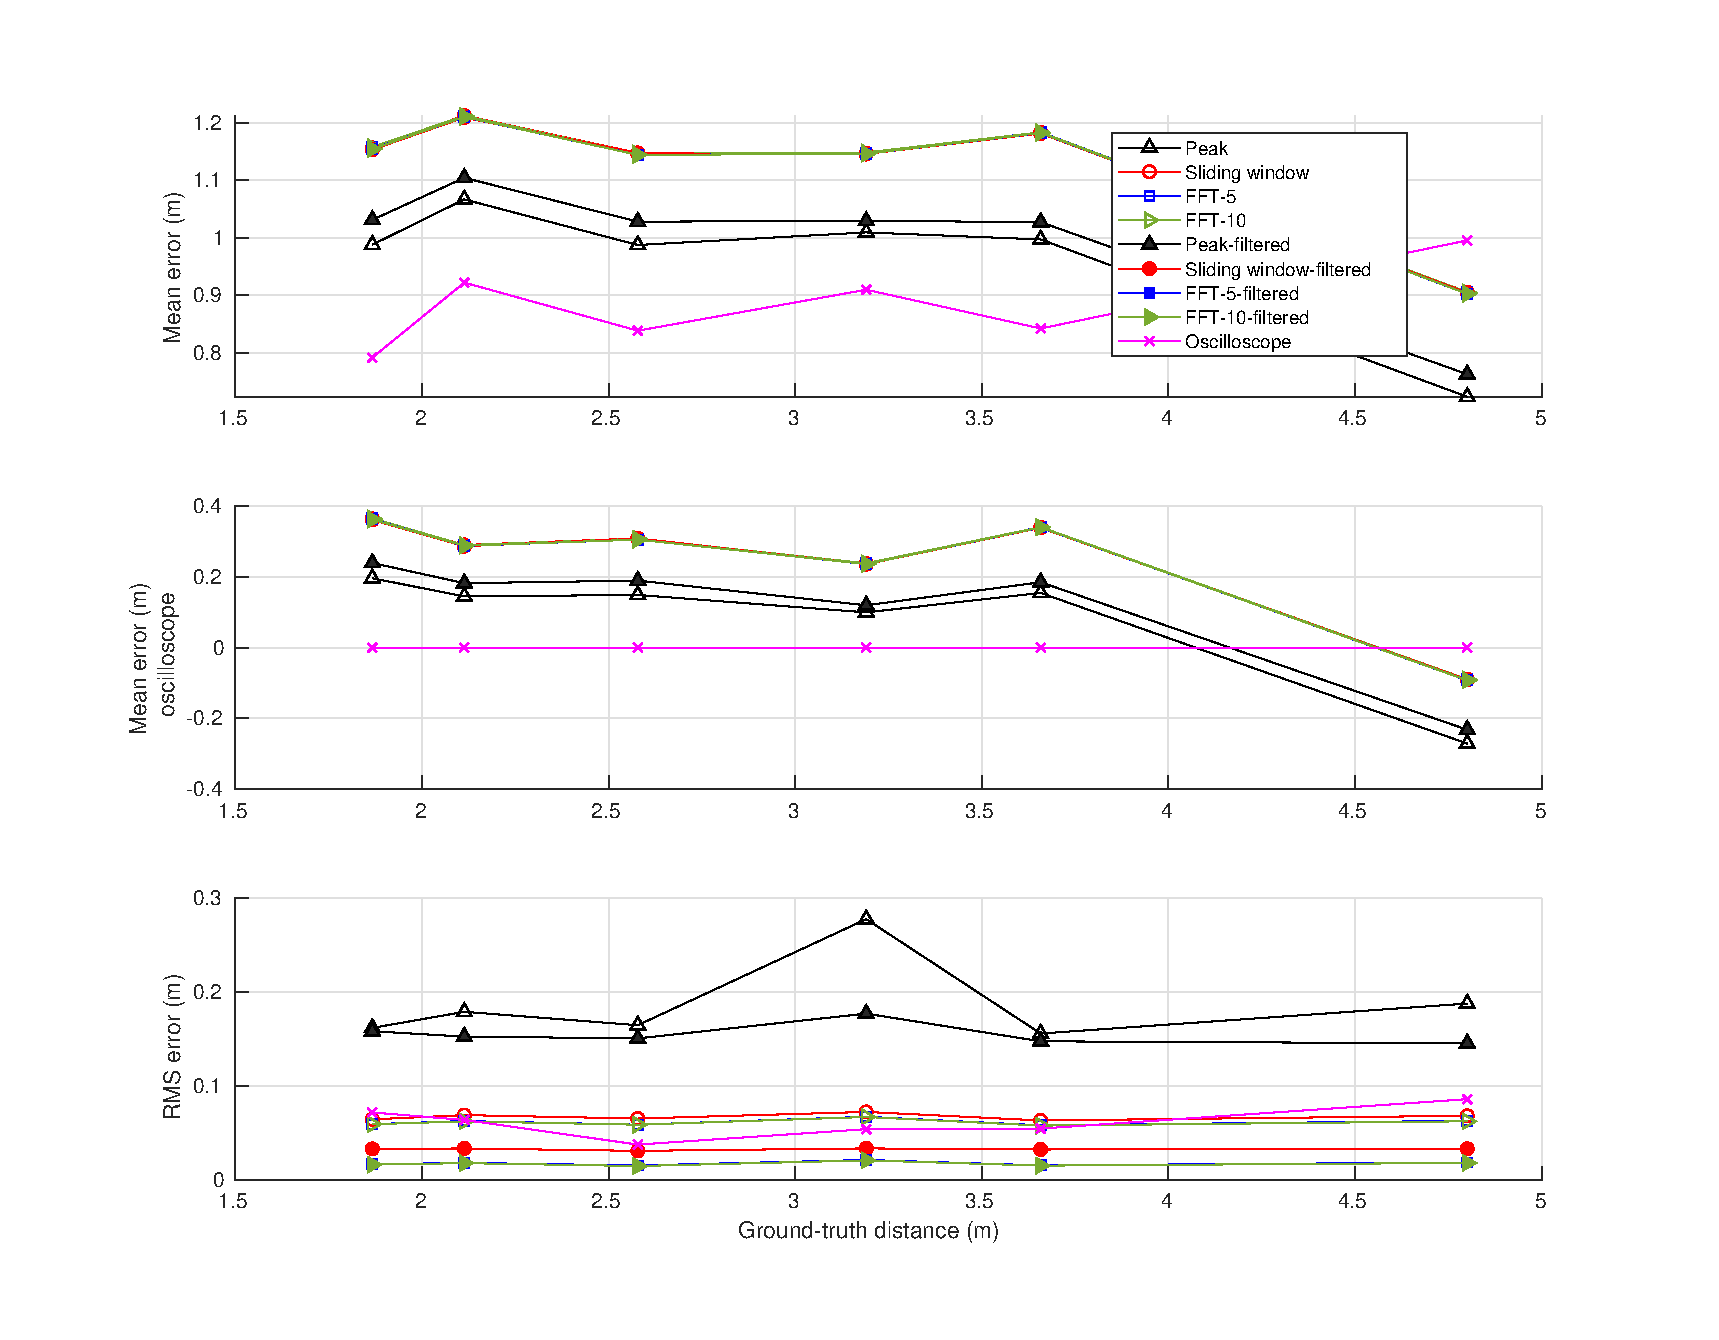
\includegraphics[width=1\textwidth]{figures/chapter_ADC_MF/Error_dist_all_FFT_real.eps}
\caption{Mean and RMS error of the NP detector using the SW and FFT approaches. The number after FFT indicates the times the resolution is refined. The hollow marker indicates the results without filtering, and the solid marker denotes the result after filtering. Figure (b) is obtained by using the distance measured by the oscilloscope signals as the reference for the mean error calculation.}
\label{fig:error_NP_real}
\end{figure}
% *****************************************************

% Application to real signal
% RMS error: (1) LP decreases the RMS error for all (2)Peak: large, Reason for large RMS of peak is that peak detection is sensitive to noise on the peak (3) conv:  FFT has less RMS than peak and sliding-conv. Because the filtered signal is still noisy so the ajacent point may have value larger than the true peak (long distance case in simulated signal). Sinsce FFT has smaller time interval, the RMS is less. 

% Mean error: (1) peak has less bias than all conv. Reason is that for 'conv', noise on the edges of a signal cause shift of the conv result (even after filtering), also the longer tail.... For, the peak detection, it is  only sensitive to noise on the peak not the ones on the edges -> no shift. (3) Peak: before vs aftre filteirng: the flat top --> right shift  (4) all conv has very similar results, the different is less than 1cm.
% ***************************************
\paragraph{Mean error}
The results of the Mean error from different estimation algorithms are shown in Figure~\ref{fig:error_NP_real}. All the estimation methods and oscilloscope measurements give positive bias of the mean distance from the ground truth distance (\ie longer distance than the ground-truth distance), which could be due to the inaccurate measurement of the ground truth. More evidence is given by the constant discrepancy between the distance measurements of the oscilloscope and the ground-truth distance. Therefore, we used the distance measured by the oscilloscope as the ground-truth in this case and the resultant mean error is shown in the Figure~\ref{fig:error_NP_real}(b). However, the positive bias still exists even though it is reduced after changing the reference, and the peak estimation gives less Mean error than the NP detectors. The positive bias could be due to the noise on the peak and the long falling edge of the measured signals. The noise could make the peak of the ground-truth signal less detectable and the long falling edge plateaus the top of the signal, which tends to move peak towards the falling edge. The different slopes of the falling edge of the transmit and return signal could also cause the shift of the peak. Specifically, for the NP detectors, in addition to the flat top of the convolution results, the convolution with asymmetric kernels and the mismatch of the shape of the kernel with each signal could be the reasons for the shift. Consequently, the right-shift of the peak will result in a larger TOF and longer distance measurement. The peak estimation algorithm has less Mean error than the NP detectors, which could be due to that the peak estimation algorithm is only sensitive to the noise on the peak while the NP detectors are depended on the noise on the whole signal and the noise on the falling edge of the signal could cause larger right shift of the convolution result. The LP-filter makes the Mean error worse than the one without filtering. The reason could be as the noise decreases, the effect of the long falling edge on the algorithm is larger than the noise at the peak which results in a larger right shift of the peak. On the other hand, different NP detectors with and without LP-filtering give similar Mean errors (difference is less than 1cm), which demonstrates effects of the noise on the peak shift of the results of the NP detector, and also shows the Mean error is dominated by the noise on the signal dominate rather than the resolution of the results even after filtering.
\todo{what is the SNR of the signal?, mentioned SNR in the discussion}
\paragraph{RMS error}
The RMS errors from different TOF estimation algorithms are shown in Figure~\ref{fig:error_NP_real}(c). The reduction of the RMS error after LP-filtering demonstrates that the capability of the low-pass filter on the removal of the 645MHz-Noise \todo{out-of-band frequency structured noise?}and improvement of the measurement precision. The RMS error of the peak estimation is worst compared to the NP detector due to the high sensitivity of the algorithm to the noise at the peak of a signal. On the other hand, among different approaches of the NP detector, the FFT-approach has less RMS error than the SW-approach. The reason could be that the signal is relatively noisy even after LP-filtering (similar to the long distance situation in the simulated signal \todo{section...}), therefore, even though variation of the peak position of the convolution result exists in both approaches, the FFT approaches with smaller sample separation provides less RMS error.\par
In the figure, we also observe the RMS error of the oscilloscope measurement is better than the peak estimation method. The reason could be that the oscilloscope has a bandwidth of 50 MHz, which works like a low-pass filter and cut off noise with frequencies higher than 50MHz, while the cut-off frequency of the applied low-pass filter is 0.4GHz. Therefore, the signal output from the oscilloscope is less noisy than the one after the LP filter, which results in a lower RMS error. \par




\subsubsection{Conclusion}
The noise at the peak of a signal needs to be treated carefully for the peak estimation algorithm and the NP detector, and a low-pass filter is a powerful way of removing any out-of-band frequency-structured noise and improve the measurement precision. Moreover, a faster clock of an ADC is required to achieve higher precision. On the other hand, to achieve a high measurement accuracy, asymmetric signals or kernel should be avoided which requires a faster detector that has a fast RC response and allows symmetric output signals.


% \section{Experiment}
% \section{ADC Information and Setup}
% 1. spec of ADC: bits, sampling rate, bw
% 2. features: remove DC, trigger modes,
% 3. exp setup: 
% \section{experiment}
% test performance of MF: 
% 1. pfa: measure noise floor of stop
% 2. pd and error: different distances, different trigger mode and length, AFE/not
% 3. ROC
% \section{Comparison of detectors}
% time cost, adv and disadv for different situations
%% Comparision between TDC and ADC



%%
% Application to real signal
% RMS error: (1) LP decreases the RMS error for all (2)Peak: large, Reason for large RMS of peak is that peak detection is sensitive to noise on the peak (3) conv:  FFT has less RMS than peak and sliding-conv. Because the filtered signal is still noisy so the ajacent point may have value larger than the true peak (long distance case in simulated signal). Sinsce FFT has smaller time interval, the RMS is less. 

% Mean error: (1) peak has less bias than all conv. Reason is that for 'conv', noise on the edges of a signal cause shift of the conv result (even after filtering), also the longer tail.... For, the peak detection, it is  only sensitive to noise on the peak not the ones on the edges -> no shift. (3) Peak: before vs aftre filteirng: the flat top --> right shift  (4) all conv has very similar results, the different is less than 1cm.


% Application to simulated data
% Mean error (1)slidng > FFT-5 > FFT-10, due to finer resolution

% RMS error (1) shorter distance sliding window < FFT. Reason is  the peak is not very noisy at shorter distance, and sliding window has coarse resolution,so  ajacent points to the peak is less likely to have competetive value to the peak. so RMS is less. For FFT, the resolution is high, so the ajacent poits could have value equal or higher than the peak, so some variaion. 

% at larger distance, the signal becomes noisy,  the adjacent points has larger fluctuation which starr to affect the sliding window, and because of the larger time interval, the RMS is larger than the variation of FFT

% (3) the LP filter remove the noise on the signal --> signal becomese smooth, so the  situation becomes similar to the short distance case: the ajacent points has less change to chanllage the peak position, so the RMS is less. Howerver, the high resol of FFT --> higher RMS. BUT, all the RMS is less than 1cm !!!


% algorithm comparsion !!!
% peak : less Mean error (less shift), but high RMS (noise on the peak). Fix of RMS: LP filter
% conv-sliding window: larger Mean error: shift(noise on the edges), less RMS (less sensitive to peak noise). Fix of Mean (higher resolution --> FFT-5/10)